%%%%%%%%%%%%%%%%%%%%%%%%%%%%%%%%%%%%%%%%%%%%%%%%%%%%%%%%%%%%%%%%%%%
%                                                                 %
%  GEANT manual in LaTeX form                                     %
%                                                                 %
%  Michel Goossens (for translation into LaTeX)                   %
%  Version 1.00                                                   %
%  Last Mod. Jan 24 1991  1300   MG + IB                          %
%                                                                 %
%%%%%%%%%%%%%%%%%%%%%%%%%%%%%%%%%%%%%%%%%%%%%%%%%%%%%%%%%%%%%%%%%%%
\Origin{R.Brun, A.McPherson, P.Zanarini}
\Revision{S.Giani}
\Documentation{P.Zanarini, S.Giani}
\Submitted {15.08.83}     \Revised{11.12.92}
\Version{Geant 3.15}\Routid{DRAW110}
\Makehead{Drawing a Volume -- Case 1}
 
\Shubr{GDRAW}{(CHNAME,THETA,PHI,PSI,U0,V0,SU,SV)}
Draws an orthographic parallel projection or
a perspective projection 
of volume {\tt CHNAME} according to the options set via the 
routine \Rind{GDOPT} and all its {\it visible} descendants
(see routine \Rind{GSATT} to alter the visibility of a volume)
at position {\tt U0,V0} (user coordinates), with the scale
factors {\tt SU} and {\tt SV};
the object is seen from {\tt THETA} and {\tt PHI} angles, and
the resulting 2D projection is rotated
by an angle {\tt PSI} on the screen plane.
These parameters, as well as zoom parameters set by \Rind{GDZOOM}
define the current {\it view parameters}, and they are copied
in the common \FCind{/GCDRAW/}. Attributes like colour, surface fill,
line width, line style, visibility, etc. can be set by calling 
the \Rind{GSATT} routine for {\tt CHNAME} and its descendants 
{\tt [GEOM 500]}. An example of the result of the call:

\begin{center}
{\tt CALL GDRAW('ARM ',40.,40.,0.,nx,ny,0.015,0.015) }
\end{center}

is given in fig~\ref{draw110-1} for various values of the attributes
and graphic options.

\begin{figure}[hbt]
      \centering
      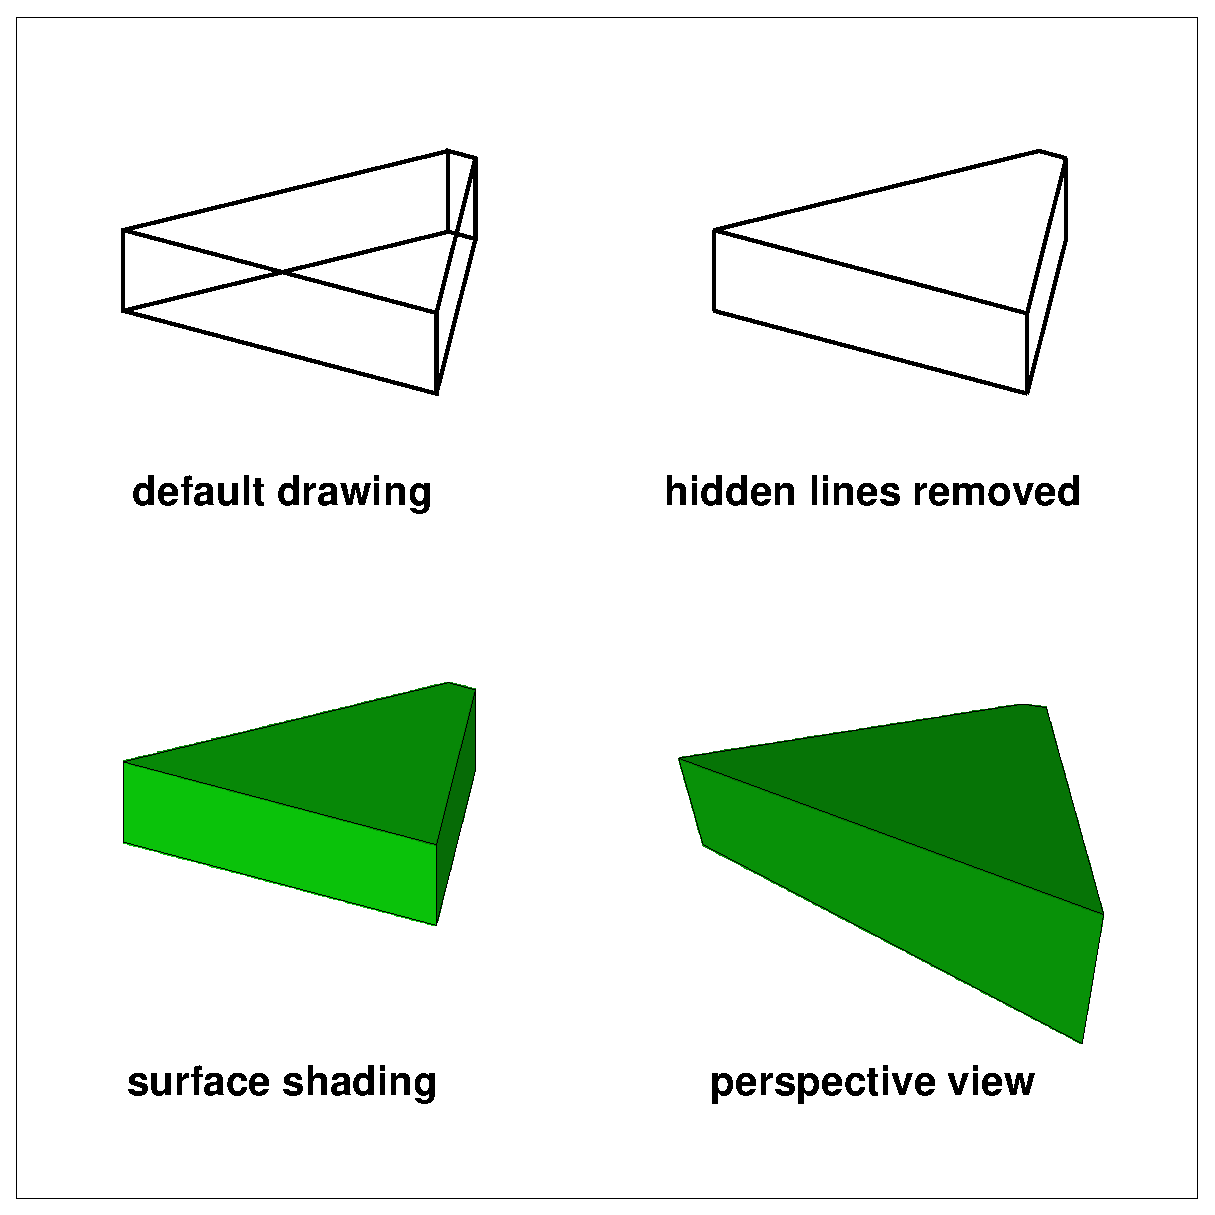
\epsfig{file=eps/draw110-1.eps,width=10cm}
      \caption{Examples of use of {\tt GDRAW}}
      \label{draw110-1}
\end{figure}

Drawing with hidden line removal and surface fill shading is also possible, 
but the drawing time may increase substantially for complicated 
objects.

When using the interactive interface it is possible to {\it cut}
the object to be drawn with {\it cutting} volumes (command {\tt CVOL}).
This is particularly
useful to visualise the contents of an object drawn with hidden line removal.
Another feature which is available only interactively is the possibility
to draw each decendant of a volume shifted along the axis which goes from the
centre of the local coordinate system to the centre of gravity of
the descendant itself. This again is useful to improve the visibility of the
details of a complicated setup (command {\tt BOMB}). Please see the interactive
interface description for more information on this part.

\begin{DLtt}{MMMMM}
\item[CHNAME]  ({\tt CHARACTER*4}) volume name.
\item[THETA] ({\tt REAL}) theta angle between the line of sight and the
Z axis of {\tt MA}ster {\tt R}eference {\tt S}ystem ({\tt MARS}).
\item[PHI]   ({\tt REAL}) phi angle between the projection of the line 
of sight on plane {\tt X  Y} and the {\tt X} axis of {\tt MARS}.
\item[PSI]   ({\tt REAL}) psi angle by which the projected image will 
be rotated on the screen plane.
\item[U0]    ({\tt REAL}) u coordinate on the screen of the volume origin.
\item[V0]    ({\tt REAL}) v coordinate on the screen of the volume origin.
\item[SU]    ({\tt REAL}) scale factor for u coordinates.
\item[SV]    ({\tt REAL}) scale factor for v coordinates.
\end{DLtt}
